\documentclass[border=4pt]{standalone}
\usepackage{amsmath,amssymb,amsfonts}
\usepackage{xcolor,colortbl,array,booktabs,multirow}
\usepackage{tikz}
\usepackage{pgfplots}
\pgfplotsset{compat=1.16}
\usetikzlibrary{arrows, automata, backgrounds, calendar, chains, decorations,
    matrix, mindmap, patterns, petri, positioning, shadows, shapes.geometric,
    trees, shapes, decorations.pathreplacing, calc, tikzmark, arrows.meta,
    intersections, fit, graphs, quotes, angles, decorations.markings}
\newcommand{\st}{\text{ s.t. }}
\newcommand{\x}{\mathbf{x}}
\renewcommand{\b}{\mathbf{b}}
\renewcommand{\c}{\mathbf{c}}
\newcommand{\A}{\mathbf{A}}
\newcommand{\y}{\mathbf{y}}
\newcommand{\z}{\mathbf{z}}
\newcommand{\R}{\mathbb{R}}
\newcommand{\RR}{\mathbb{R}}
\newcommand{\Z}{\mathbb{Z}}
\newcommand{\ZZ}{\mathbb{Z}}
\newcommand{\npcomplete}{NP-complete}
\providecommand{\true}{\text{TRUE}}
\providecommand{\false}{\text{FALSE}}
\tikzset{vertex/.style={circle,fill=black!25,minimum size=20pt,inner sep=0pt},
    edge/.style={draw,thick,-},weight/.style={font=\small},
    selected vertex/.style={vertex, fill=red!24},
    selected edge/.style={draw,line width=2pt,-,red!50},
    ignored edge/.style={draw,line width=2pt,-,black!20}}
\newcommand{\vect}{\vec}
\providecommand{\ds}{\displaystyle}
\providecommand{\longvect}{\overrightarrow}
\usepackage[normalem]{ulem}
\definecolor{ocre}{RGB}{243,102,25}
\providecommand{\leftB}{\left[}
\providecommand{\rightB}{\right]}
\tikzset{directed/.style={postaction={decorate,decoration={markings,mark=at position .65 with {\arrow{>}}}}},
    directed1/.style={postaction={decorate,decoration={markings,mark=at position .65 with {\arrow{>}}}}}}
\begin{document}
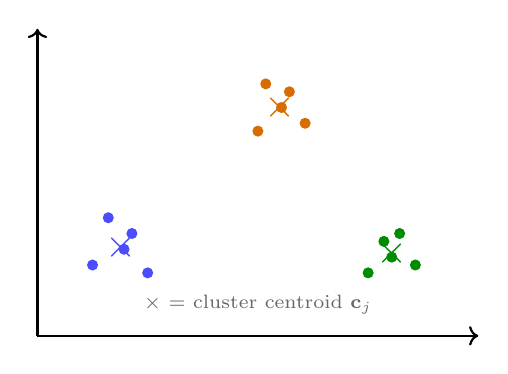
\begin{tikzpicture}[scale=1.0]
  \draw[->, thick] (0,0) -- (5.6,0);
  \draw[->, thick] (0,0) -- (0,3.9);
  % cluster A (blue) around (1,1)
  \foreach \x/\y in {0.7/0.9, 1.2/1.3, 0.9/1.5, 1.4/0.8, 1.1/1.1}
    \fill[blue!70] (\x,\y) circle (2pt);
  \node[blue!70, font=\Large] at (1.06,1.12) {$\times$};
  % cluster B (orange) around (3,2.9)
  \foreach \x/\y in {2.8/2.6, 3.2/3.1, 3.4/2.7, 2.9/3.2, 3.1/2.9}
    \fill[orange!85!black] (\x,\y) circle (2pt);
  \node[orange!85!black, font=\Large] at (3.08,2.9) {$\times$};
  % cluster C (green) around (4.5,1.05)
  \foreach \x/\y in {4.2/0.8, 4.6/1.3, 4.8/0.9, 4.4/1.2, 4.5/1.0}
    \fill[green!55!black] (\x,\y) circle (2pt);
  \node[green!55!black, font=\Large] at (4.5,1.04) {$\times$};
  \node[font=\scriptsize, text=black!60] at (2.8,0.4) {$\times$ = cluster centroid $\mathbf{c}_j$};
\end{tikzpicture}
\end{document}
